% Use class option [extendedabs] to prepare the 1-page extended abstract.
\documentclass[extendedabs]{bmvc2k}
\usepackage[colorlinks = true,
            linkcolor = blue,
            urlcolor  = blue,
            citecolor = blue,
            anchorcolor = blue]{hyperref}
\usepackage{kotex} % 한국어 사용 가능

% Document starts here
\begin{document}
\title{Accelerating the Super-Resolution Convolutional Neural Network}
\addauthor{
Lee Gwan Hui$^1$, \today}{}{1}
\addinstitution{
$^1$2017142136, Department of Electrical and Electronic Engineering, Yonsei University.}
\maketitle
\let\thefootnote\relax\footnote{This is an extended abstract. The full paper is available at the \href{https://github.com/LeeGwanHui/TIL/tree/main/deeplearning_ham}{github}. }
\vspace{-0.2in}

\section{abstract}

\quad Super-Resolution이란 저해상도(Low resolution) 이미지를 고해상도(High resolution)로 변환시키는 문제로 2가지 접근 방법이 있다.\cite{youtube}
크게 Supervised learning 방식과 GAN을 활용해 고해상도 이미지를 생성하는 방식이다. 이 예비 보고서에서는 Supervised learning 중에서도 CNN을 이용한 초기
모델인 SRCNN을 발전시킨 FSRCNN을 살펴볼 것이다. 
이 논문의 motivation은 SRCCNN은 이미 성능이 좋지만 real-time에 사용하기에는 computational cost가 높다는 점을 해결하는 것이다.
 즉 이 논문의 목적은 SRCNN의 속도를 높인 구조를 제안하는 것으로 크게 3가지를 중심으로 다룰 것이다. 
 첫째, network 끝단의 deconvolution layer을 삽입하는 것이다.
 두번째, SRCNN의 mapping layer에 shrinking layer와 expanding layer을 삽입하는 것으로 layer의 depth는 깊게 쌓되 계산량은 적게 설계한다.
 마지막으로, smaller filter size을 채택하는 것이다.
 결론적으로, 이 제안된 모델은 real-time에도 동작하기 위해서 SRCNN보다 압도적으로 speed up을 성취하였고 performance는 비슷하거나 약간 더 좋다.
 
 \subsection{introduction}
 \quad SRCNN은 간단한 구조와 좋은 restoration quality 때문에 주목을 받았다. 하지만 기존의 learning-based method보다 빠름에도 큰 이미지에서 processing speed가 
 여전히 불만족 스럽다는 단점이 있었다. SRCNN 보다 적어도 17배의 speed up이 일어나야 24fps인 real-time에 사용할 수 있다.
 이 문제를 해결하기 위해서 
 첫번째로, SRCNN에서 pre-processing step으로 upsampling하는 과정을 생략하고 마지막에 deconvolution layer로 upsampling을 진행하였다.
 두번째로, 위의 과정 때문에 감소한 정확도를 보안하기 위해 shrinking layer와 expanding layer로 사용해서 parameter의 
 급격한 증가 없이 non-linear mapping layer의 depth를 늘렸다. 다음장부터 FSRCNN의 형태를 살펴볼 것이다.
 이 논문의 목표는
 첫번째로, compact hourglass-shape CNN structure을 제안해서 빠른 image super-resolution을 진행하는 것이다.
 두번째로는 제안된 모델이 real-time에도 사용할 수 있도록 FSRCNN을 재구조화(FSRCNN-s)하는 것이다.
 
 \subsection{Fast Super-Resolution by CNN}
 \quad \textbf{SRCNN} 이 논문은 SRCNN을 발전시킨 모델이기 때문에 먼저 SRCNN \cite{dong2015image} 을 이해해야 한다. 이 논문은 Super-resolution의
 판도를 딥러닝 기반으로 바꾼 모델를 제안하였는데 SRCNN은 성능이 좋지만 단지 real-time에 쓸 수 없다는 단점이 있다.
 \newline  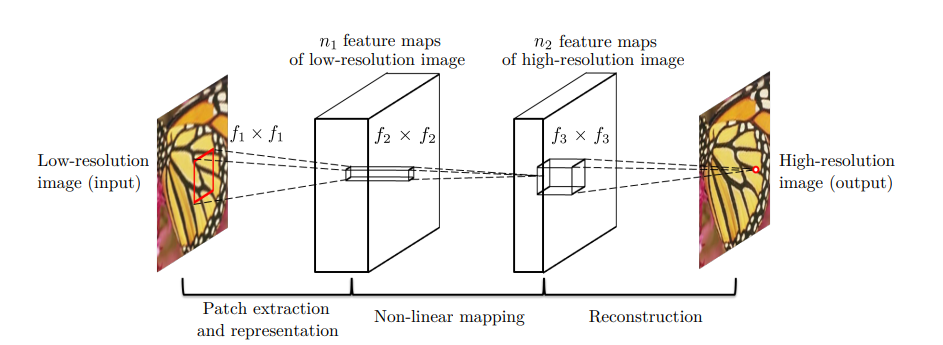
\includegraphics[width=\linewidth]{images/00_SR.PNG}
 SRCNN의 구조는 3가지 영역 Patch extraction and representation, Non-linear mapping 그리고 Reconstruction 로 되어 있다.
 먼저 Patch extraction의 경우에는 bicubic interpolation을 진행한 input image에서 patches을 뽑는 과정이다.
 두번째로 통과하는 non-linear mapping의 경우에는 non-linearity를 추가하는 것으로 neural network의 depth을 늘리는 과정으로 볼 수 있다.
 마지막으로 Reconstruction에서는 앞서 만들어진 patches를 모아 high-resolution image을 만든다. 
 이렇게 단 Convolutional layer 3개로 모델을 설정하였다. 이 때 성능을 비교해봐도 다른 deeplearning algorithm을 쓰지
 않은 방식에 비해 성능이 더 좋다. 
 \newline  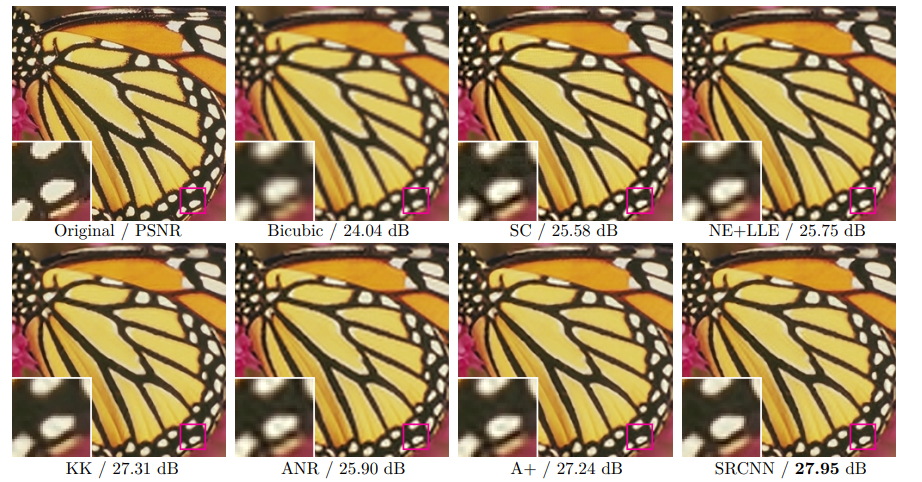
\includegraphics[width=\linewidth]{images/01_SR.PNG}
 이를 적용한 계산 복잡도는 $O\{({f_i}^2n_1+n_1{f_2}^2n_2+n_2{f_3}^2)S_{HR}\}$로 나타낼 수 있다. 여기서  ${{\{f_i\}}^3}_{i=1}$ 과 ${{\{n_i\}}^3}_{i=1}$은 각각
 filter size 와 filter number of three convolution layers을 나타낸다. 그리고 $S_{HR}$는 size of the HR image 이다.      
 \newline SRCNN이 real-time에 쓰일 수 없는것은 크게 두가지 이유로
 이미지를 전처리하는 과정에서 bicubic interpolation을 사용해 upsampling을 먼저 진행하기 때문에 큰 feature size가 CNN layer 전역에서 돌아다니며 계산하게 된다.
 또한, non-linear mapping step에서 높은 channel 수(dimension)를 유지하며 CNN을 통과하기 때문에 정확도는 높지만 계산량이 증가하는 결과를 초래한다.
 \newline 위의 한계점을 개선한다면 계산 속도가 상승할 것이다. 그렇기 때문에 이를 해결하여 real-time에서 사용하기 위한 FSRCNN이 개발된 것이다.
 \newline \quad \textbf{FSRCNN} 논문에 핵심 architecture인 FSRCNN \cite{dong2016accelerating}을 살펴보자. 총 5개의 part로 순서대로 feature extraction, shrinking, mapping,
 expanding, deconvolution 으로 구성되어 있다. 아래 그림을 참고하자.
 \newline  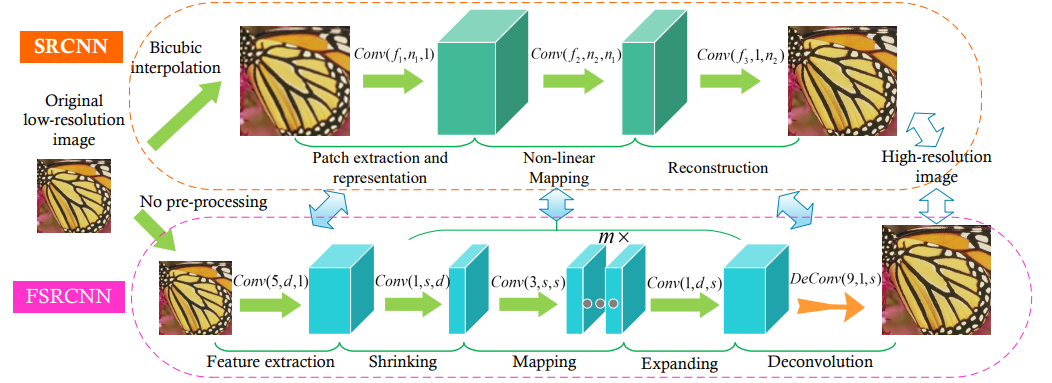
\includegraphics[width=\linewidth]{images/02_SR.PNG}
 이 논문에서 성능과 속도에 영향을 심각하게 미치는 variable을 sensitive variable이라고 정의한다. 구조를 살펴보면서 하나씩 정의해 나갈 것이다.
 FSRCNN의 구조에 들어가기 앞서 convolution layer을 $Conv(f_i,n_i,c_i)$ 라고 정의하고 deconvolution layer은 $DeConv(f_i,n_i,c_i)$ 라고 정의한다. 
 순서대로 kernel size, output channel 수, input channel 수이다. 
 \newline \quad \textbf{feature extraction} 제일 처음 소개할 구조는 feature extraction이다. SRCNN의 Patch extraction and representation과 비슷한
 형태지만 input image에 전처리로 bicubic interpolation을 사용하지 않는다는 점에서는 다르다. kernel의 크기는 interpolation을 하지 않은 image이므로 feature size가 작기 때문에 5면 충분하다. 이를 표현하자면 
 $Conv(5,d,1)$ 로 표현할 수 있다. 
 여기서 d는 위에서말한 sensitive variable로 클수록 정확도는 증가하지만 계산량이 많아져 일종의 trade off 관계에 있는 parameter이다.
 \newline \quad \textbf{Shrinking} 두번째로 소개할 구조는 Shrinking layer이다. 이 부분은 계산량을 감소시키기 위한 trick으로 non-linear mapping을 하기전에 실시한다.
 1x1 convolution layer을 통해 channel 수를 줄이게 되어 다음과 같이 표현할 수 있다. $Conv(1,s,d)$.
 여기서 s는 sensitive variable이다.
 \newline \quad \textbf{Non-linear mapping} 이 부분은 SRCNN에도 있는 구조지만 SRCNN에서는 오직 single non-linear mapping을 사용했다. 특히 FSRCNN에서는
 매우 중요한 layer인데 SRCNN과는 다르게 interpolation을 하지 않아서 정확도 측면에서 부족한 상태이기 때문에 cnn의 depth를 늘려 정확도를 높여줘야한다.
 $ m \times Conv(3,s,s) $로 표현할 수 있다.
 여기서 m은 sensitive variable이다.
 \newline \quad \textbf{Expanding} 여기서는 shrinking layer에서 축소한 channel을 다시 복구 시키는 곳이다. expanding layer없이 upsampling 시키면 정확도 측면에서 효율이 좋지 못하다.
  즉 이 구조를 넣은 이유는 대칭적인 구조가 더 성능이 좋게 나왔기 때문이라고 할 수 있다. $ Conv(1,d,s) $ 로 쓸 수 있다.
 \newline \quad \textbf{Deconvolution} FSRCNN의 핵심이 되는 부분이다. deconvolution을 이해하기 위해서는 convolution 개념으로부터 접근하는 것이 좋다.
 \newline  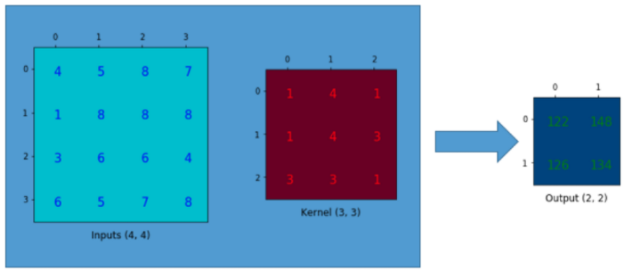
\includegraphics[width=\linewidth]{images/03_SR.PNG}
 위의 convolution layer은 4x4 feature size를 가지고 있는 input에 대해서 kernel size가 3이고 stride가 1인 convolution filter을 통과시킨다면 결과가 2x2 matrix가 나온다는 것을 보여준다.
 이 연산 과정 중 kernel을 matrix로 표현한다면 \cite{deconv} 아래와 같이 표현가능하다.
 \newline  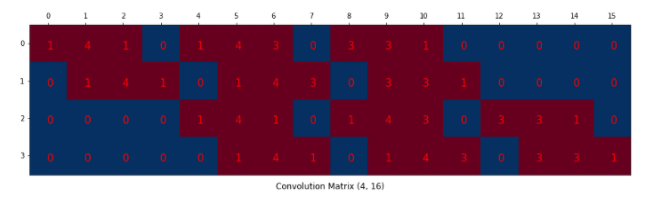
\includegraphics[width=\linewidth]{images/04_SR.PNG}
 위 그림의 의미는 kernel을 matrix로 표현한 것으로 이를 이용해서 Y=AX 의 matrix 연산으로 표현하면 아래와 같이 표현할 수 있다. 
 \newline  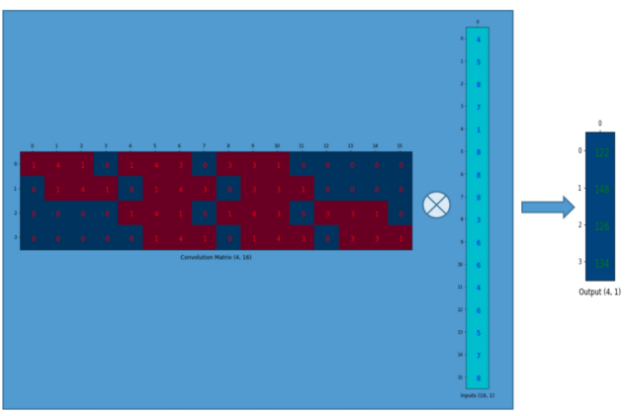
\includegraphics[width=9cm, height=4cm]{images/05_SR.PNG}
 \newline 즉 이런 convolution 과정을 통해서 output matrix인 2x2를 flatten한 형태의 결과를 얻을 수 있다는 것이다.
 이제 볼것은 deconvolution으로 여기까지 따라왔으면 이해할 수 있다. 이제 과정은 2x2 matrix에서 4x4 matrix를 얻어야 한다. 이를 일종의 upsampling으로도 볼 수 있다. 
 즉 flatten한 vector의 형태로는 각각 4x1과 16x1의 vector을 얻으면 된다. 이는 A를 transform 시킨 $A^T$을 이용하면 된다.
 \newline  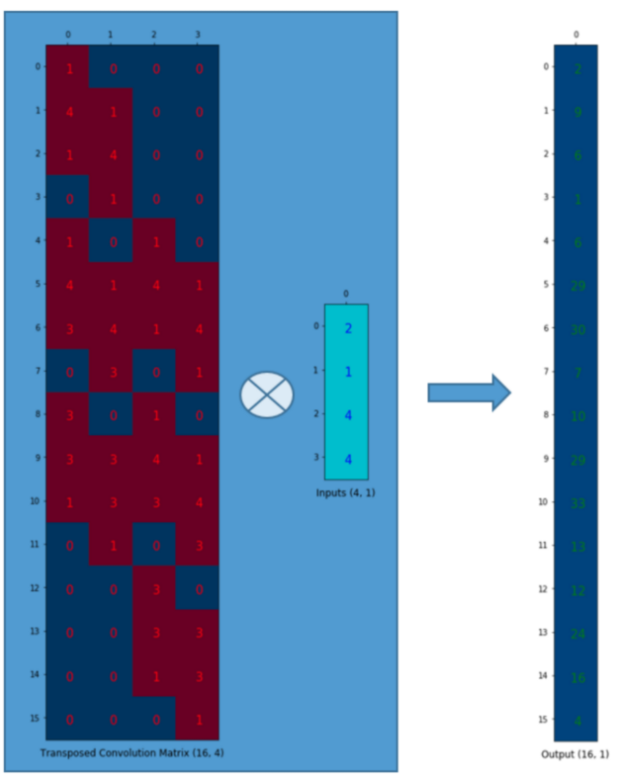
\includegraphics[width=9cm, height=6cm]{images/06_SR.PNG}
 \newline 이런 방식으로 deconvolution layer이 진행된다. 이런 deconvolution은 명명상 Transposed convolution이 더 적합하다고 한다.
 \newline 이제 다시 돌아가서 FSRCNN에서의 적용을 살펴보자. FSRCNN에서는 deconvolution layer을 upsampling에 이용하고 이전 layer의 output feature을 종합하는 역할을 한다.
 식으로 나타내면 $ DeConv(9,1,d) $로 나타낼 수 있다. 
 \newline \quad \textbf{추가적인 특징} deconvolution layer을 마지막으로 FSRCNN의 구조는 끝이 났지만 학습을 위해 사용한 몇가지 테크닉에 대해 소개해볼까한다.
 이 논문에서는 ReLU의 zero gradients에 의해 야기되는 dead features을 PReLU을 사용해서 예방한다. 또한 cost function으로는 MSE을 사용한다.
 \newline \quad \textbf{overall structure}
 전체적인 구조는 $ Conv(5,d,1) - PReLU - Conv(1,s,d) - PReLU - m \times Conv(3,s,s) - PReLU - Conv(1,d,s) - PReLU - DeConv(9,1,d) $ 이다.
 특히 sensitive variable을 이용해서 FSRCNN(d,s,m)으로 표기한다. 이 실험으로 얻는 계산 복잡도는 $ O\{(9ms^2+2sd+106d)S_{LR}\}$ 이다.
 여기서 주목할 점은 위의 SRCNN의 계산복잡도는 HR image size에 비례하지만 FSRCNN은 original LR image size에 비례하게 complexity가 결정된다는 것이다. 
 이는 SRCNN은 interpolation을 진행했고 FSRCNN은 input image를 바로 사용하기 때문이다. 
 \newline \quad \textbf{SRCNN vs FSRCNN}
 앞에서도 수없이 언급했지만 마지막으로 두개의 차이를 정리해보자. 먼저  deconvolution layer로 upscaling 진행하는 차이점이 있다.
 또다른 차이로는 SRCNN에서는 single mapping layer이었던 반면 FSRCNN에서는 shrinking layer,4 mapping layers and an expanding layer로 구성을 바꾸었다.

 \subsection{Experiments}
 실험 결과를 보기전에 PSNR의 정의가 필요하다. 
 \newline 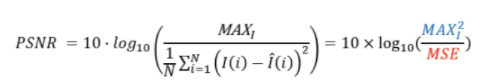
\includegraphics[width=\linewidth]{images/08_SR.PNG}
 여기서 말하는 $MAX_i$는 일반적인 이미지에서 255값을 의미하는 값이고 MSE는 $\frac{1}{N}\sum_{i=1}^{N}{(I(i)-\hat{I}(i))}^2$ 을 의미한다.
 여기서 I(i)는 원본 이미지 픽셀값을 의미하고 $\hat{I}(i)$는 예측이미지 픽셀값을 나타낸다. 즉 원본이미지 픽셀값과 예측 이미지 픽셀값이 같게 되면 MSE=0이 되어 최댓값을 알 수 없다.
 PSNR은 원본 이미지 대비 손실된 품질의 정도를 파악하는 것으로 보통 40이 넘어가면 잘 복원되었다고 평가한다.
 \newline 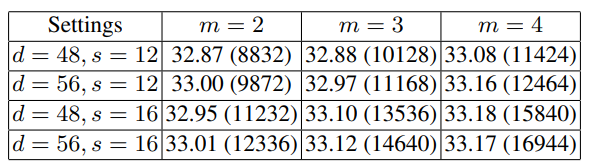
\includegraphics[width=\linewidth]{images/07_SR.PNG}
 위의 테이블은 sensitive variable을 변화시켜 PSNR의 값을 비교하기 위해 나타낸 것이다. 괄호안의 값은 parameter의 수를 나타낸다.
위의 테이블을 보면 m(Non-linear mapping layer 수)이 클수록 더 좋은 성능을 낸다. 이는 cnn layer의 depth가 증가하기 때문이다. 
또한 d와 s가 증가할 수록 정확도가 증가하는 경향을 보이는데
이를 해석하자면 더 많은 channel로 처리할 수록 더 많은 image의 feature을 추출하기 때문에 성능이 좋아진다. 
\subsection{Conclusion}
 이 논문에서는 계산량을 극단적으로 줄인 변형된 FSRCNN-s 모델을 만들어 real-time에도 돌릴 수 있고 의미있는 성능을 가진 모델을 제시하였다.
 아래 그림은 이전에 유명한 SR model들과 비교해서 FSRCNN은 가장 좋은 성과를 얻은 것을 보여준다.
 즉 이 논문의 성과는 이전의 논문들보다 성능이 좋고 더 계산량이 작아 real-time에도 사용할 수 있는 모델을 만들었다는 것이 가장 크다. 이 논문에서는 이를 성취하기 위해서
 deconvolution layer의 개념을 사용하였고 또한 계산량을 줄이기 위해 1x1 convolution layer도 사용하였다. 
 \newline 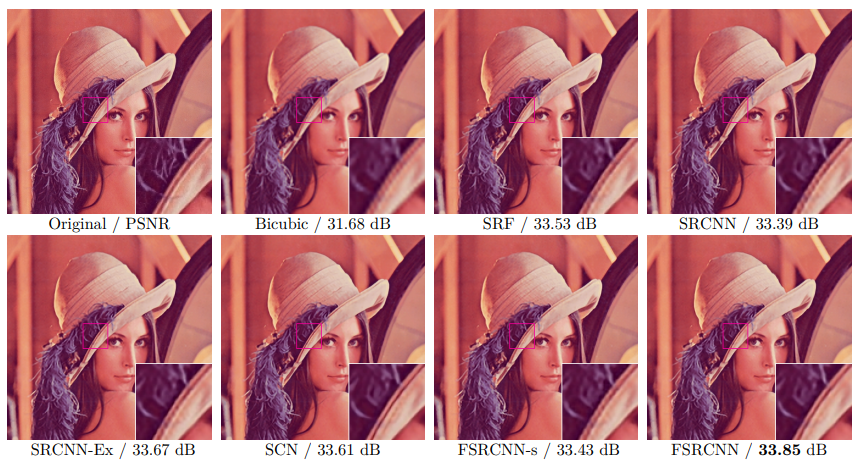
\includegraphics[width=9cm, height=4cm]{images/09_SR.PNG}

\newpage
\bibliography{egbib}

\end{document}
